\documentclass[12pt]{article}

\usepackage{url}
\usepackage{fullpage}
\usepackage{amssymb,amsfonts}
\usepackage{amsmath}
\usepackage{amsthm}
\usepackage[normalem]{ulem}
\usepackage{graphicx}

\begin{document}

\title{Process Book}
\author{Moritz Winger}
\maketitle

\section{Project Description}

Medical Store GeoChallenge: see http://databits.io/challenges/medical-store-geospatial-challenge

The main questions posed by the challenge are:

\begin{itemize}
\item Over time, is there a tendency for customers from a particular referral source to come from a specific Toronto metro
area? This can help achieve geographic targeting of marketing efforts.

\item  Over time, what are the referral trends per customer source and in comparison with other sources?
This can help understand what referral source is more effective than others.

\item Over time, is there a tendency for customers from particular referral sources to get bundles of products, or return
to the store for more products or services? This can help understand which referral source helps build a more loyal
customer base.
\end{itemize}


\section{Data}

Data sets have been provided: A data set on referrers with their geographical data and the number of clients
referred to the medical store and time-resolved data on client visits with number of purchased articles and client
geo-data.

The provided data sets are enough to answer the three questions with appropriate representation.

\section{Design Iterations}

\begin{itemize}

\item Design iteration 1

\begin{center}
\scalebox{0.6}{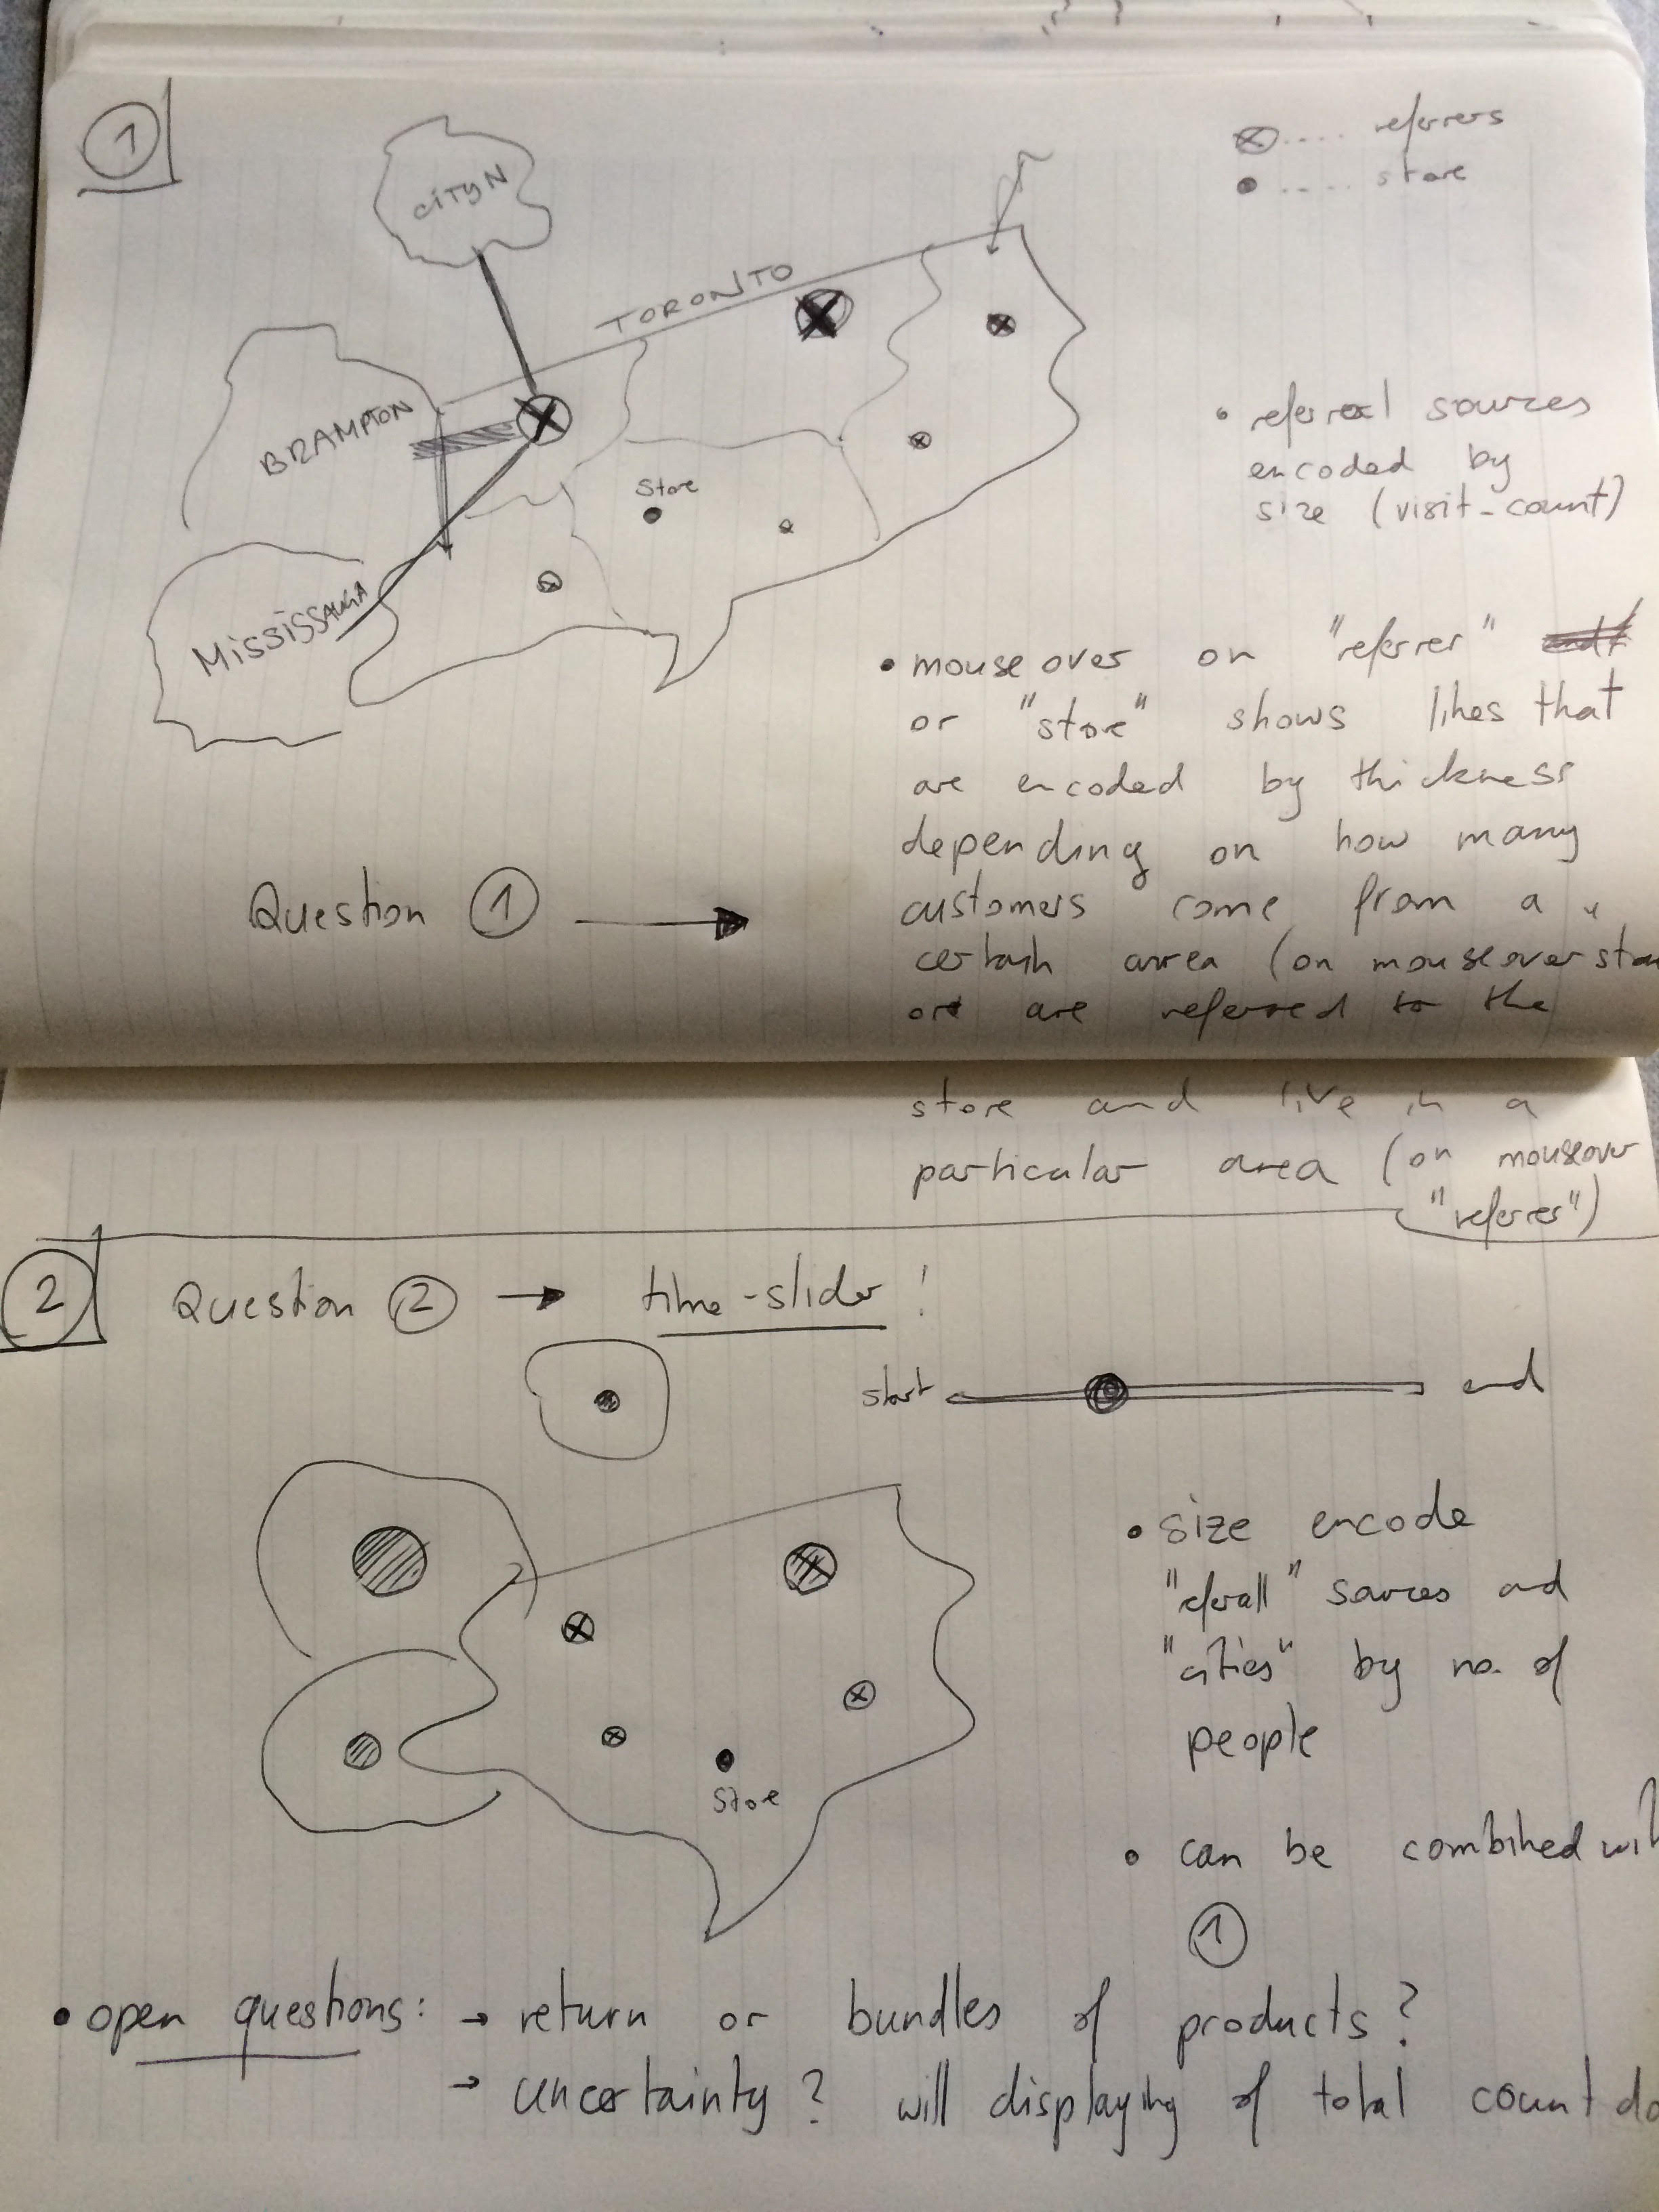
\includegraphics[scale=0.25]{Design_sketches_iteration_1}} \\
\end{center}

The first design proposition was a visualization that shows all clients and referrers on a map and allows
interaction on hovering the mouse over a client or referrer. By this type of interaction, the viewer can
extract total and time-averaged quantities such as total visits, visits per client, total purchased items, etc.

To address the question on time-resolved properties, the visualization would also have a time-slider, where
properties are shown as a function of time.

A simple implementation of this feature, however showed that the data was to sparse to efficiently populate
the graph (map) and properly visualize the desired quantities. ALso it would have been hard to compare quantities
at different points in time.

\item Design iteration 2

\begin{center}
\scalebox{0.6}{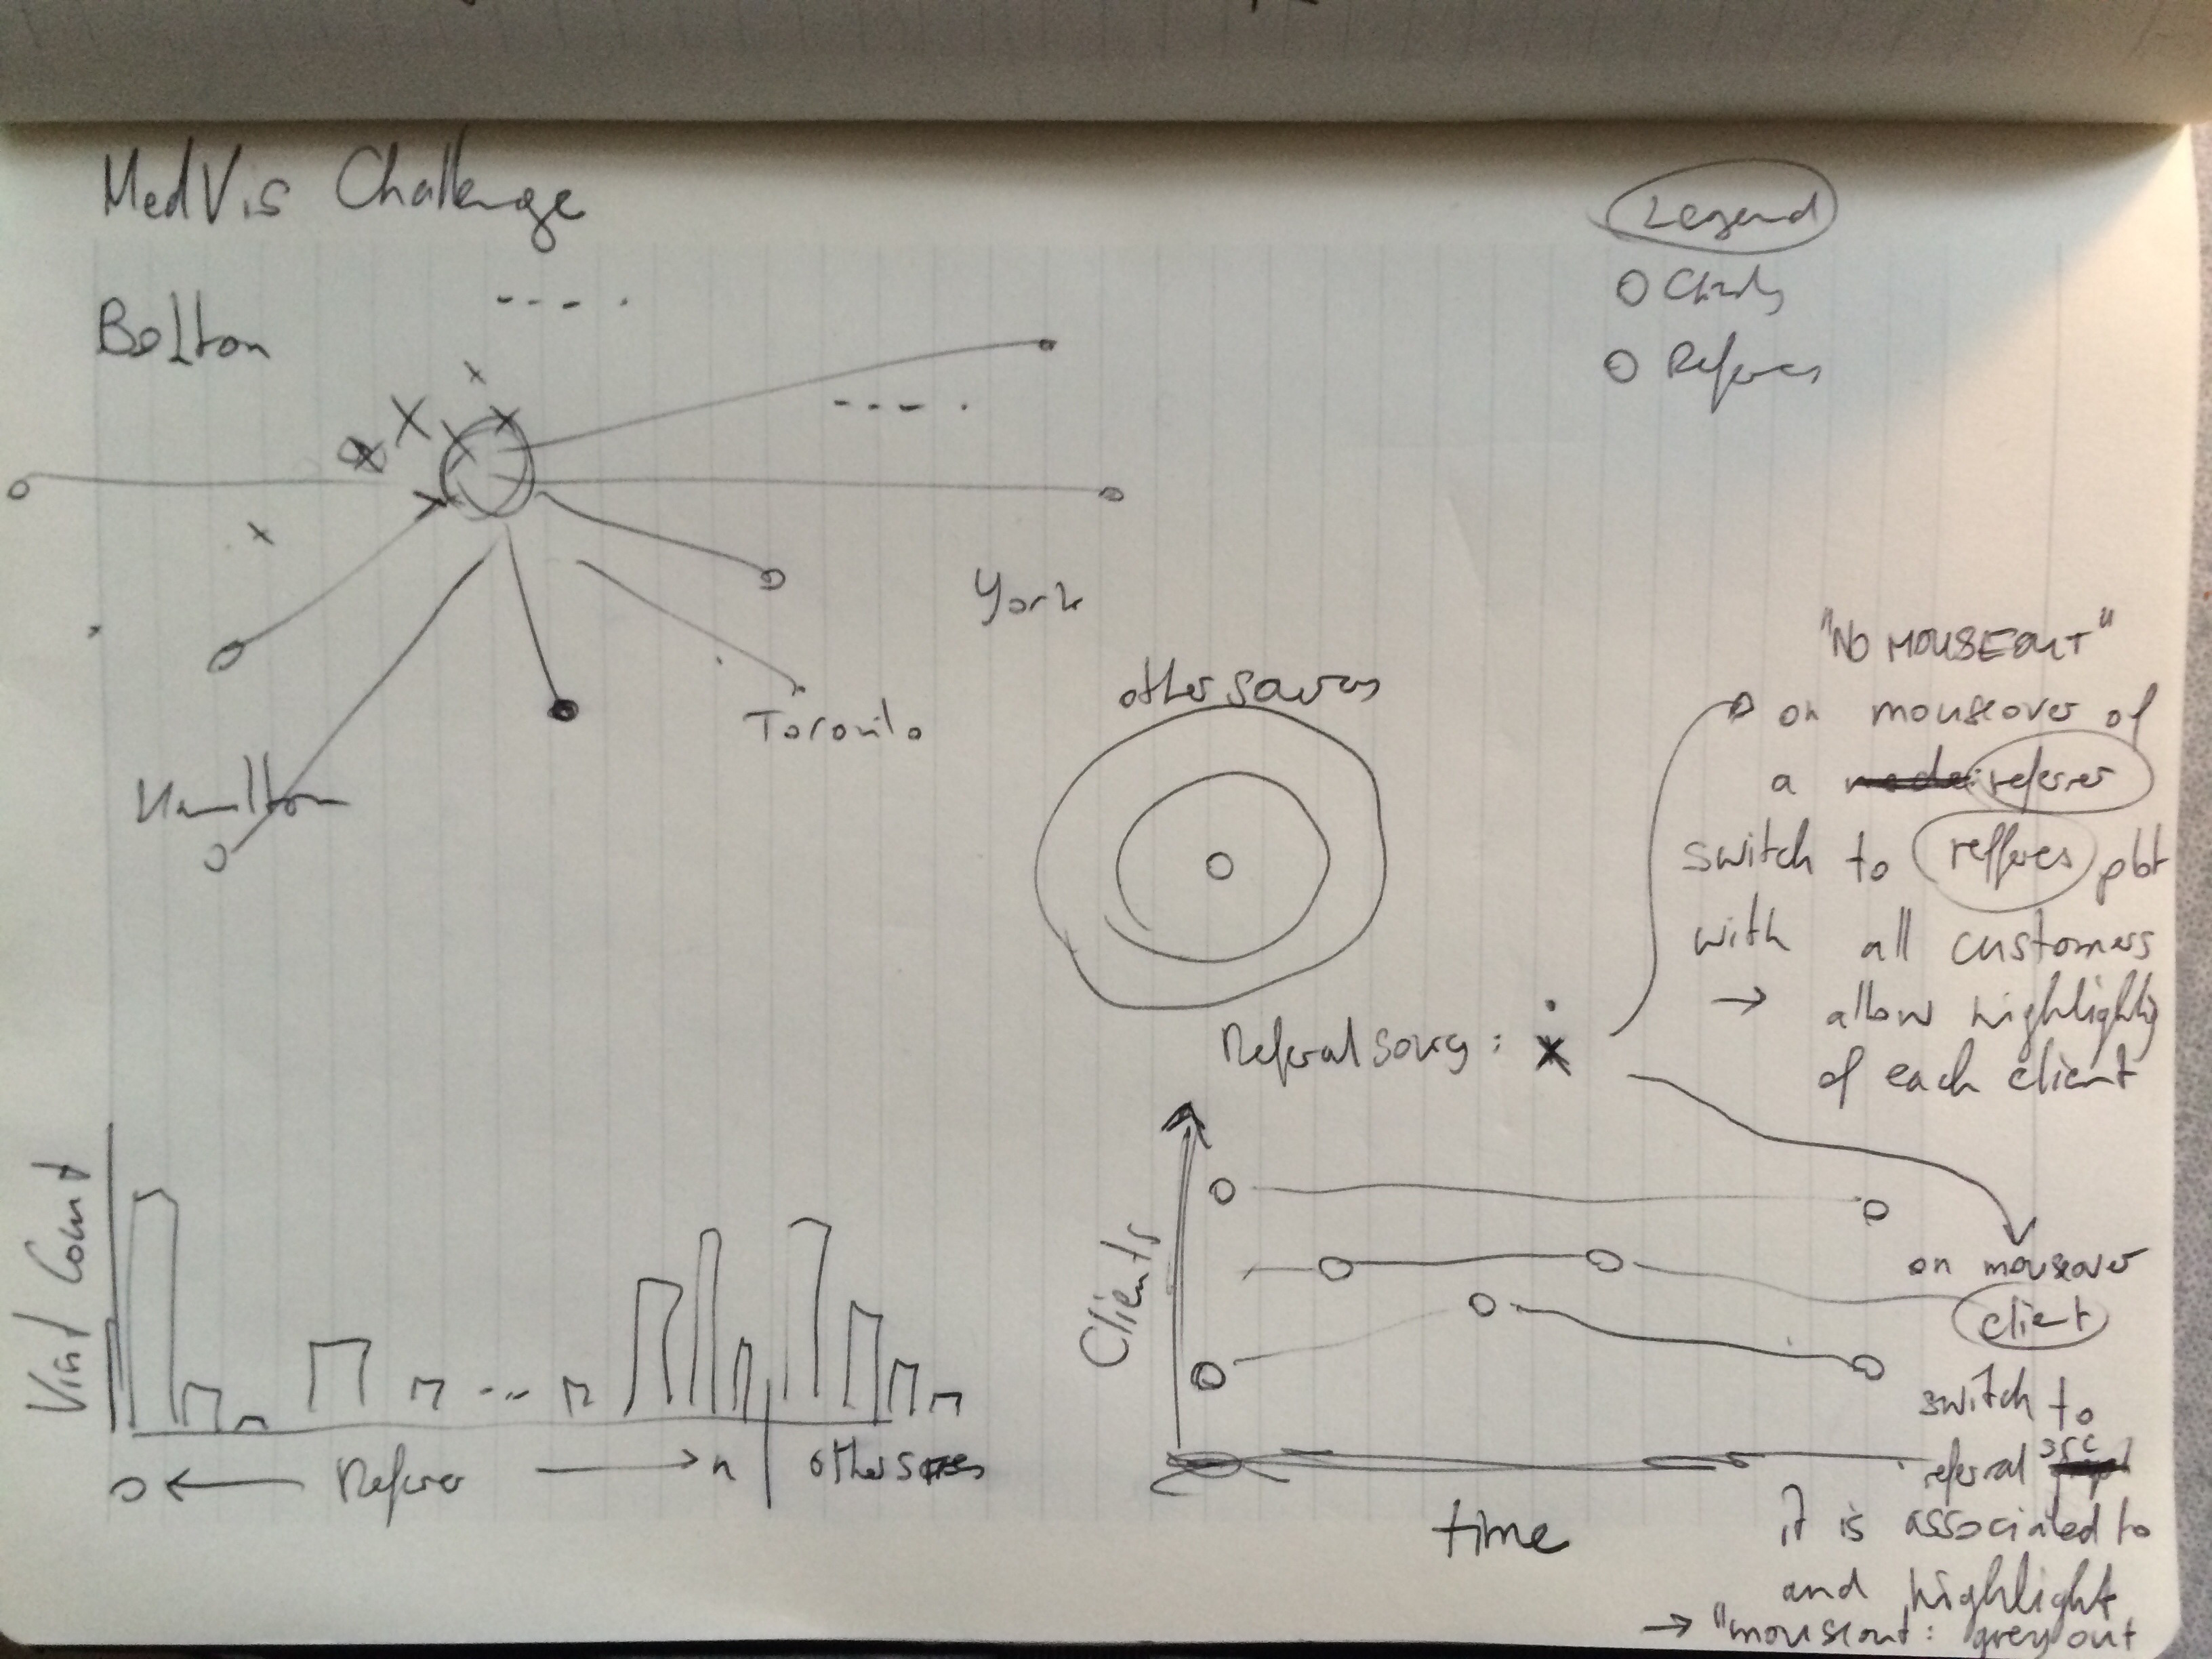
\includegraphics[scale=0.2]{Design_sketches_Milestone_1}} \\
\end{center}

In this iteration, a clearer design concept has been developed with a simple theme and color coding to distinguish
clients and referrers. The general concept of having a map to visualize the client / referrer distribution has been
kept but reduced to a simple graph representation that suited well the developed design concept.
Because of problems with the time-slider as discussed above, the idea has been discarded and an additional visual
element has been created, namely the time resolved visualization of purchase events per referral source.
In addition, to quantify where clients on the map have been referred from, a simple barchart has been constructed to
easily distinguish popular referral sources from the others.
The idea of size-encoded circles has been implemented.

\item Design iteration 3

Visual elements in text form have been added to display referrer and client data on a detailed level, whenever a
referrer or client element is selected anywhere in the visualization. This allows analysis on a finer resolution:
Inspecting the map visual element, we get an overview over referrer sources and clients,  looking at the time visualization we get a clear idea of how clients from a particular referral source behave. The visual element developed 
in this iteration gives the user the actual values of the datapoint selected.

\item Final Design

\begin{center}
\scalebox{0.6}{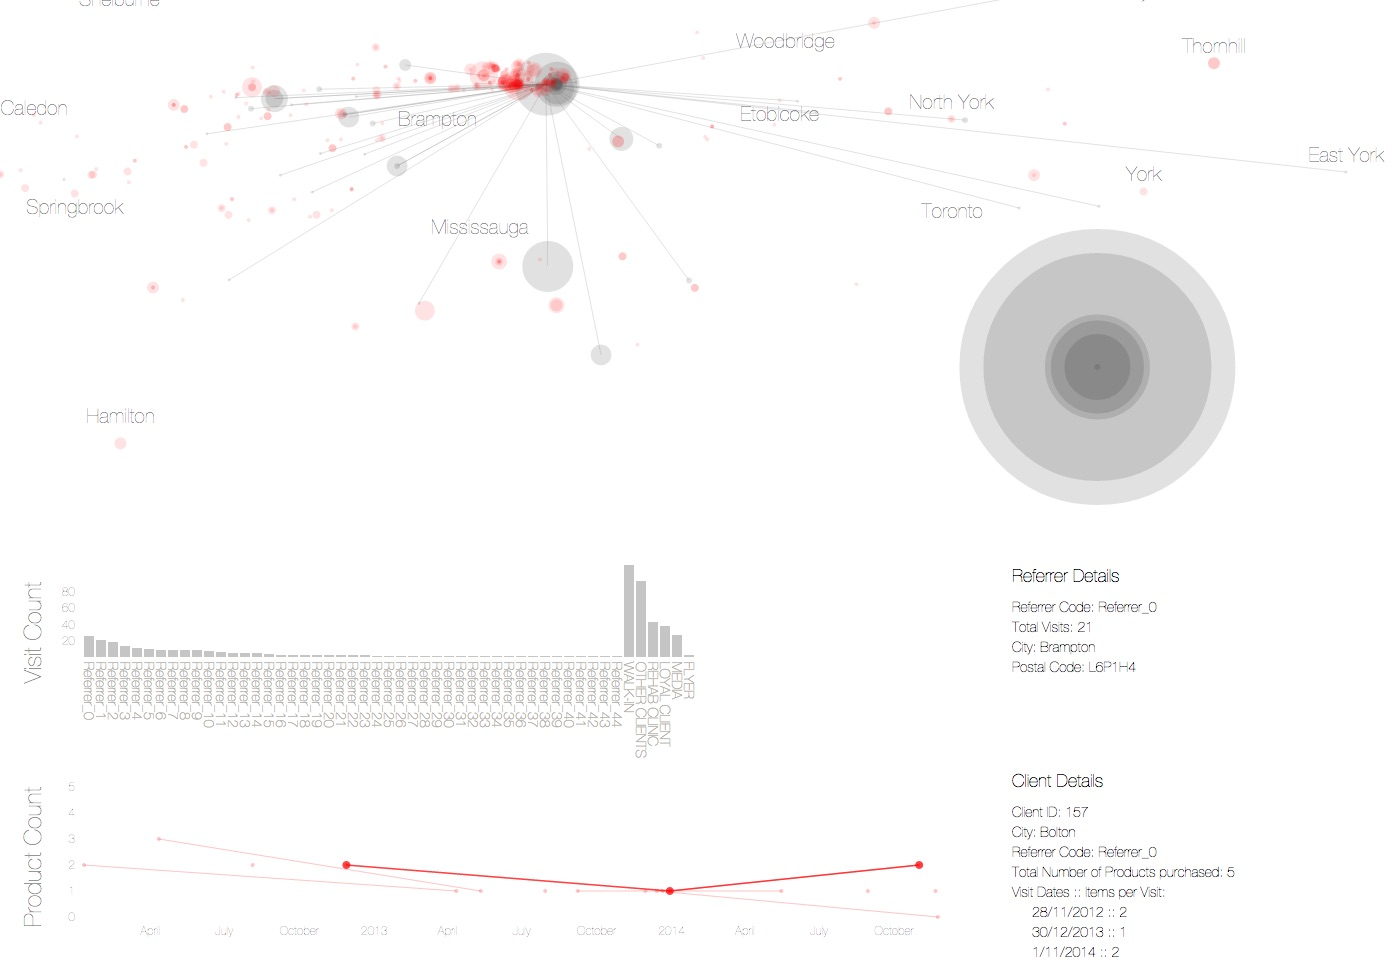
\includegraphics[scale=0.5]{Screenshot_vis}} \\
\end{center}

The final design combines all the elements developed in the previous iteration and includes appropriate interactivity to be triggered by
user's mouse movement.

\section{Analysis}

The intention of the presented visualization was to make the provided data accessible without much explanation. The focus of the visualization 
lies in simplicity and interactivity to study the data in the viewer's own pace.

The three questions posed are addressed in the different elements of the vis.

Question 1 is mostly covered by the graph visualization (scatter plot), we can select a referral source and we get the associated clients highlighted immediately. In addition, we can hover over the clients and see the city they are from highlighted in the map and also in the detail visualization on the bottom right.
To study Question 2 the viewer may be referred to the barchart to see how many customers come from a particular referral source, as well as the time visualization, when he selects a referral source. The clients from this referral source are shown in the graph, the viewer is able to conceive how many times a client has visited and how many items were purchased. Details can be viewed when hovering over a client circle or line.
Question 3 is addressed by the time visualization, where we see the buying behaviour of all customers (returning?, number of products, time). Additional info on particular clients, such as exact visit dates and number of purchased items per visit, we get from the client detail view. Through the time visualization graph the user also gets a qualitative description of the dataset's uncertainty.


\end{document}